\subsection{Featureauswahl}
\label{sec:feature_selection}
Untersucht wurden die Features aus Tabelle \ref{tab:songFeatures} die von Song et al. genutzt wurden, das Motion History Image und 2 selbst entwickelte Features. Die Features aus
Tabelle \ref{tab:songFeatures} erfüllen ohne Änderungen nicht ausreichend Anforderungen. Die Features 2, 5 und 7 bis 9 wurden nicht getestet, da sie sehr komplexe Berechnungen bedürfen.
\newline
\newline
Das \textit{Mean absolute value} Feature ermöglicht die einzelnen Handgesten zu unterscheiden, wenn das Feature auf verschiedene Zeitfenster dupliziert wird. Zusätzlich kann die Helligkeit normalisiert werden.
Um die Featuremenge zu verringern, können Spalten und Zeilen zusammengefasst werden. In der Praxis generalisierte der Ansatz aber nicht gut. Es wird vermutet, dass die Varianz sehr groß ist, wenn die
Handgeste mit verschiedenen Geschwindigkeiten ausgeführt wird.
\newline
\newline
\textit{Average amplitude change} eignet sich gut, um horizontale und vertikale Bewegungen zu unterscheiden. Allerdings ist es nicht möglich symethrische Bewegungen zu unterscheiden, da die Berechnung
unabhängig von der Richtung ist. Dadurch wäre zum Beispiel eine Links nach Rechts Bewegung nicht von einer Rechts nach Links Bewegung zu unterscheiden. Aus diesem Grund wurde dieses Feature nicht
weiter untersucht.

\subsubsection{Motion History}
Das Motion History Feature komprimiert die Bewegung vieler Bilder in ein Bild, indem kürzlich stattgefundene Bewgungen heller erscheinen als länger zurückgliegende Bewegungen. Das Feature ist invariant
gegenüber unterschiedliche Lichtverhältnisse, solange die Funktion, um Bewegungen zu detektieren, $\psi$ invariant ist. Überlappende Bewegungen können nicht dargestellt werden, da die Historie überschrieben
wird. In dieser Arbeit ist das bei den validen Handgesten kein Problem, da diese keine überlappenden Bewegungen beinhalten.
\newline
\newline
Die Aussagekraft des Features ist abhängig von den Parametern $\tau$ und $\delta$. Je nach dem, ist eine Bewegungshistorie nicht sichtbar, da $\delta$ zu gering ist oder $\tau$ zu groß, oder ein Teil der
Bewegungshistorie ist abgeschnitten, da $\delta$ zu groß ist oder $\tau$ zu klein. Um dieses Problem zu umgehen, wird $\delta$ abhängig von $\tau$ und der Gestenlänge gemacht, damit die vollständige
Bewegung abgebildet wird, d. h. $\delta = \frac{\tau}{\#Bilder}$.
\newline
\newline
Eine Bewegung in einem Pixel $q$ wird durch die Funktion \ref{formular:motion_history_phi} signalisiert. Die Bewegung in $q$ findet statt, wenn eine absolute Veränderung oberhalb des Durchschnitts der
absoluten Veränderung in der Helligkeit detektiert wird.
\begin{align}
    \phi(q,t) = \begin{cases}
                    1 & if \Delta_{q,t} \geq \frac{1}{N} \sum_{n=1}^N \Delta_{q,n} \\
                    0 & otherwise
    \end{cases}
    \hspace{0.5cm}where\ \Delta_{q,t} = |q_t - q_{t-1}|
    \label{formular:motion_history_phi}
\end{align}

\subsubsection{Helligkeitsverteilung}
Die Helligkeitsverteilung stellt die Pixel mit Extrema in der Helligkeit über Zeitfenster dar. Das Extrema der Helligkeit ist entweder der hellste oder dunkelste Pixel in einem oder mehrerer Bilder. Pixel
sind heller, wenn ihre Werte größer sind und dunkler, wenn ihre Werte geringer sind. Folglich können die Pixel mit den Extrema über die Komposition der Funktionen $\arg$ und $\max$ bzw. $\min$ definiert werden,
d. h. für ein Bild $Q$ ist der hellste Pixel $q' = \arg(\max Q)$ und der dunkelste Pixel $q' = \arg(\min Q)$.
\newline
\newline
Eine Handgeste besteht aus einer Sequenz von Bildern. Diese wird in Zeitfenster unterteilt, sodass möglichst gleich viele Bilder in jedem Zeitfenster enthalten sind. Ist die Anzahl der Bilder nicht ohne
Rest teilbar für die Anzahl der Zeitfenster, so werden die überschüssigen Bilder uniform auf die Zeitfenster verteilt. Anschließend wird jedes Zeitfenster zusammengefasst. Es gibt mehrere Möglichkeiten
die einzelnen Bilder in einem Zeitfenster zusammenzufassen.
\begin{itemize}
    \item Wähle das Minimum bzw. Maximum.
    \item Projeziere die Pixel der Extrema auf ein kartesisches Koordinatensystem und fasse die Punkte über eine Abstandsmetrik zusammen, z. B. über den euklidischen Abstand.
    \item Unterteile die Pixel der Extrema in Quadranten und wähle den Quadranten, der die meisten Einträge hat.
\end{itemize}
Außerdem können die Anzahl der Zeitfenster variiert werden und Pixel zu Gruppen zusammengefasst werden, d. h. Spalten und Zeilen. In der Variation dieses Features, das ausgewählt wurde, wird aber
keine Gruppierung vorgenommen. Es werden 6 Zeitfenster extrahiert, die über die Projektion der Pixel der Extrema auf ein kartesisches System über den euklidischen Abstand zusammengefasst werden.
\newline
\newline
Es wird davon ausgegangen, dass dieses Feature invariant gegenüber unterschiedlichen Lichtverhältnissen ist, da nur relative Helligkeitsunterschiede Relevant sind und Kontraste irrelevant sind bei der
Berechnung.

\subsubsection{Schwerpunktverteilung}
\label{sec:schwerpunktverteilung}
Die Schwerpunktverteilung stellt Schwerpunkte über Zeitfenster dar. Der Schwerpunkt $(X_Q, Y_Q)$ in einem Bild $Q$ (Formel \ref{formular:pictureAsFormular}) ist über die Helligkeit der einzelnen
Pixel definiert. Der Pixel $q_{11}$ bildet den Nullpunkt des Koordinatensystems. Dann ist relativ zur Gesamthelligkeit $P = \sum_{i,j} q_{i,j}$, $X_Q=\frac{\sum_{i=0}^{2} q_{i,2} - \sum_{i=0}^{2} q_{i,0}}{P}$
die horizontale Komponente und $Y_Q = \frac{\sum_{i=0}^{2} q_{0,i} - \sum_{i=0}^{2} q_{2,i}}{P}$ die vertikale Komponente des Schwerpunktes \cite{schwerpunktAnsatz}.
\begin{figure}
    \centering
    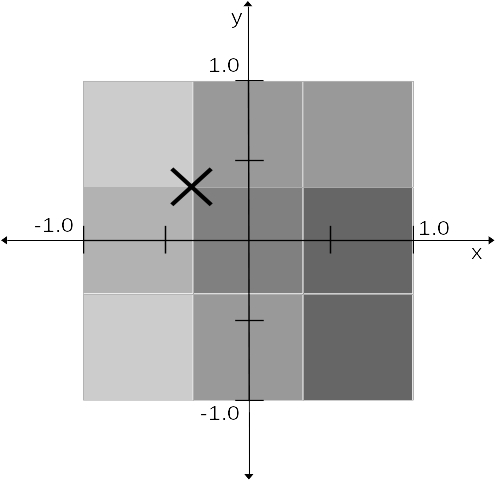
\includegraphics[width=0.5\linewidth]{images/schwerpunkt_ansatz.jpg}
    \caption{Illustration des Schwerpunktes im 3x3 Fotowiderstand-Array.}
    \label{fig:schwerpunkt}
\end{figure}
\begin{align}
    Q = \begin{pmatrix}
            q_{00} & q_{01} & q_{02} \\
            q_{10} & q_{11} & q_{12} \\
            q_{20} & q_{21} & q_{22}
    \end{pmatrix}
    \label{formular:pictureAsFormular}
\end{align}
Die Handgeste wird in Zeitfenster aufgeteilt. Jedes Zeitfenster beinhaltet gleich viele Bilder. Sollte die Anzahl der Bilder nicht ohne Rest mit der Anzahl der Zeitfenster teilbar sein, werden der
Rest uniform auf die Zeitfenster verteilt.
\newline
\newline
Es wurden unterschiedliche Anzahlen an Zeitfenster getestet. Entschieden wurde sich letztlich um 5 Zeitfenster, da einerseits die Berechnung des Features mit zunehmender Zeitfensteranzahl komplexer wird
(Kapitel \ref{sec:eval_speed}) und andererseits zu viele Zeitfenster Redundanz erzeugt.
\newline
\newline
Die Schwerpunktverteilung ist durch die Dividierung mit $P$ invariant gegenüber Skalierung der Helligkeit, jedoch nicht gegenüber einem Offset. Alternativ kann $P$ weggelassen werden, damit ausschließlich
mit Ganzzahlen gerechnet wird. Dadurch können größere Bäume generiert werden (Kapitel \ref{sec:eval_size}) und die Feature-Extrahierung ist schneller (Kapitel \ref{sec:eval_speed}). Die Schwerpunktverteilung
mit Ganzzahlen ist durch das weglassen von $P$ invariant gegenüber einen Offset $O$, da $\sum_{i=0}^{2}(q_{i,2} + O) - \sum_{i=0}^{2}(q_{i,0} + O)\ =\ \sum_{i=0}^{2} q_{i,2} - \sum_{i=0}^{2} q_{i,0} = X_Q$
ist und analog für $Y_Q$. Der Ansatz mit den Ganzzahlen konstruiert Schwerpunkte in $[-3072, 3072]^2$ und der Ansatz mit Gleitkommazahlen konstruiert Schwerpunkte in $[-1, 1]^2$.
